\documentclass[11pt]{article}
\usepackage[a4paper, margin=1in]{geometry}
\usepackage{graphicx}
\usepackage{float}
\usepackage{amsmath}
\usepackage{amssymb}
\usepackage[font=small,labelfont=bf]{caption}
\usepackage[hidelinks]{hyperref}

\setlength{\parindent}{0pt}
\pagestyle{plain}

\title{\vspace{-2.5em}Supporting Figures\\
\large Mid-Award Progress Report: Multi-Modal Foundation Model for LArTPC Reconstruction}
\author{Omar Alterkait}
\date{}

\begin{document}
\maketitle
\vspace{-1.5em}

Liquid Argon Time Projection Chamber (LArTPC) data comprise two streams: ionization charge on
the Time Projection Chamber (TPC) wire planes, and scintillation light on the Photon Detection
System (PDS). Signal amplitudes are quoted in analog-to-digital converter (ADC) counts. The
figures below show the denoising-and-compression front-end developed this period, first for the
TPC wire planes (Figures 1--3) and then for the PDS light detectors (Figures 4--6).

\begin{figure}[H]
    \centering
    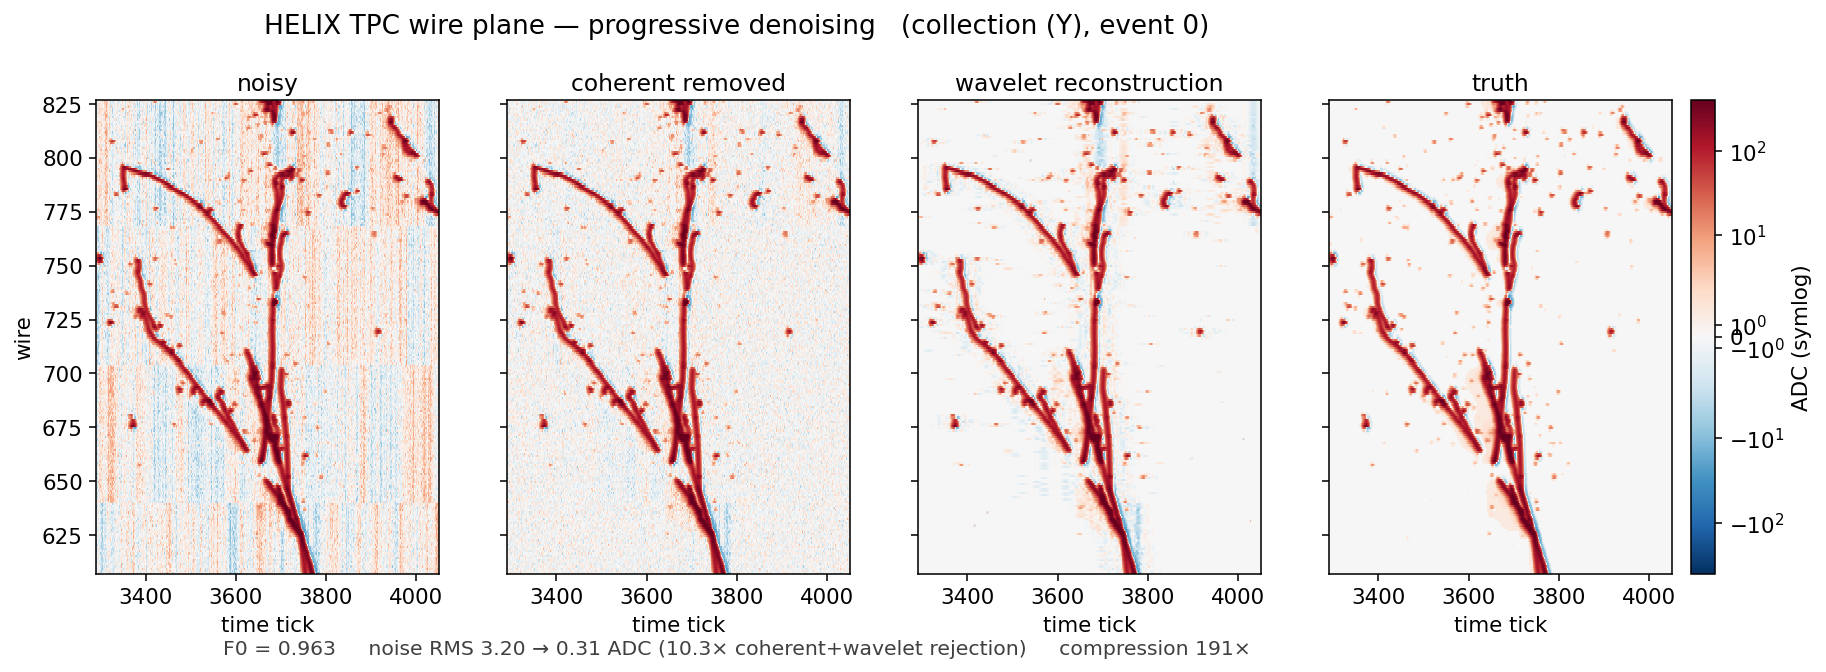
\includegraphics[width=\linewidth]{figures/tpc_denoise_Y.png}\\[4pt]
    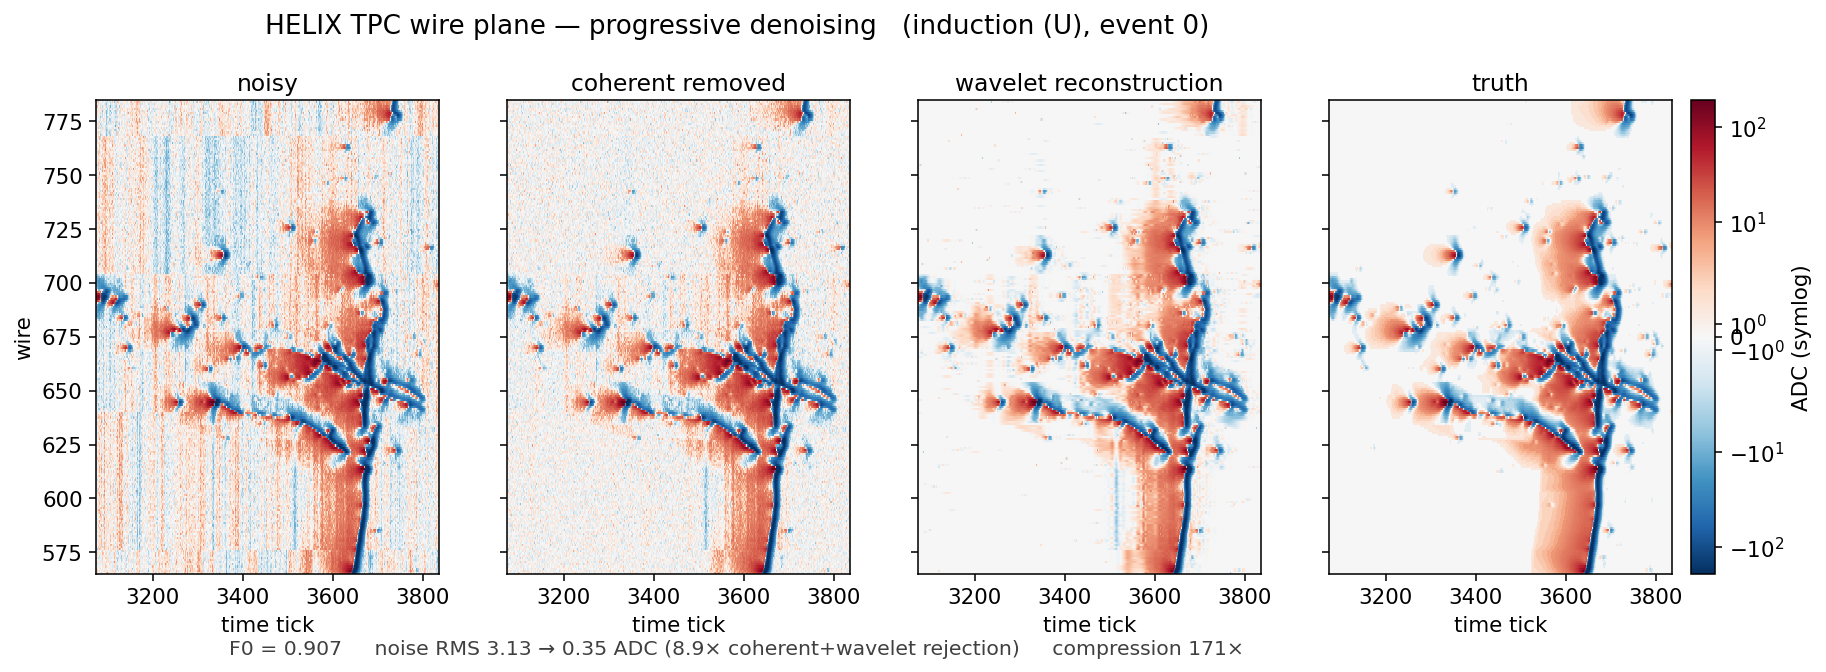
\includegraphics[width=\linewidth]{figures/tpc_denoise_U.png}
    \caption{\textbf{Progressive denoising of the TPC wire planes}, for a collection plane
    ($Y$, top row) and an induction plane ($U$, bottom row). From left to right: the raw noisy
    detector image; after coherent-noise removal; after wavelet reconstruction; and the
    noise-free simulation truth. Coherent removal eliminates the vertical correlated striping,
    and the wavelet step suppresses the remaining noise (RMS from about 3.2 to 0.3 ADC counts)
    while preserving the particle tracks. Charge fidelity is 0.96 (collection) and 0.91
    (induction), at about $190\times$ and $170\times$ compression respectively.}
\end{figure}

\begin{figure}[H]
    \centering
    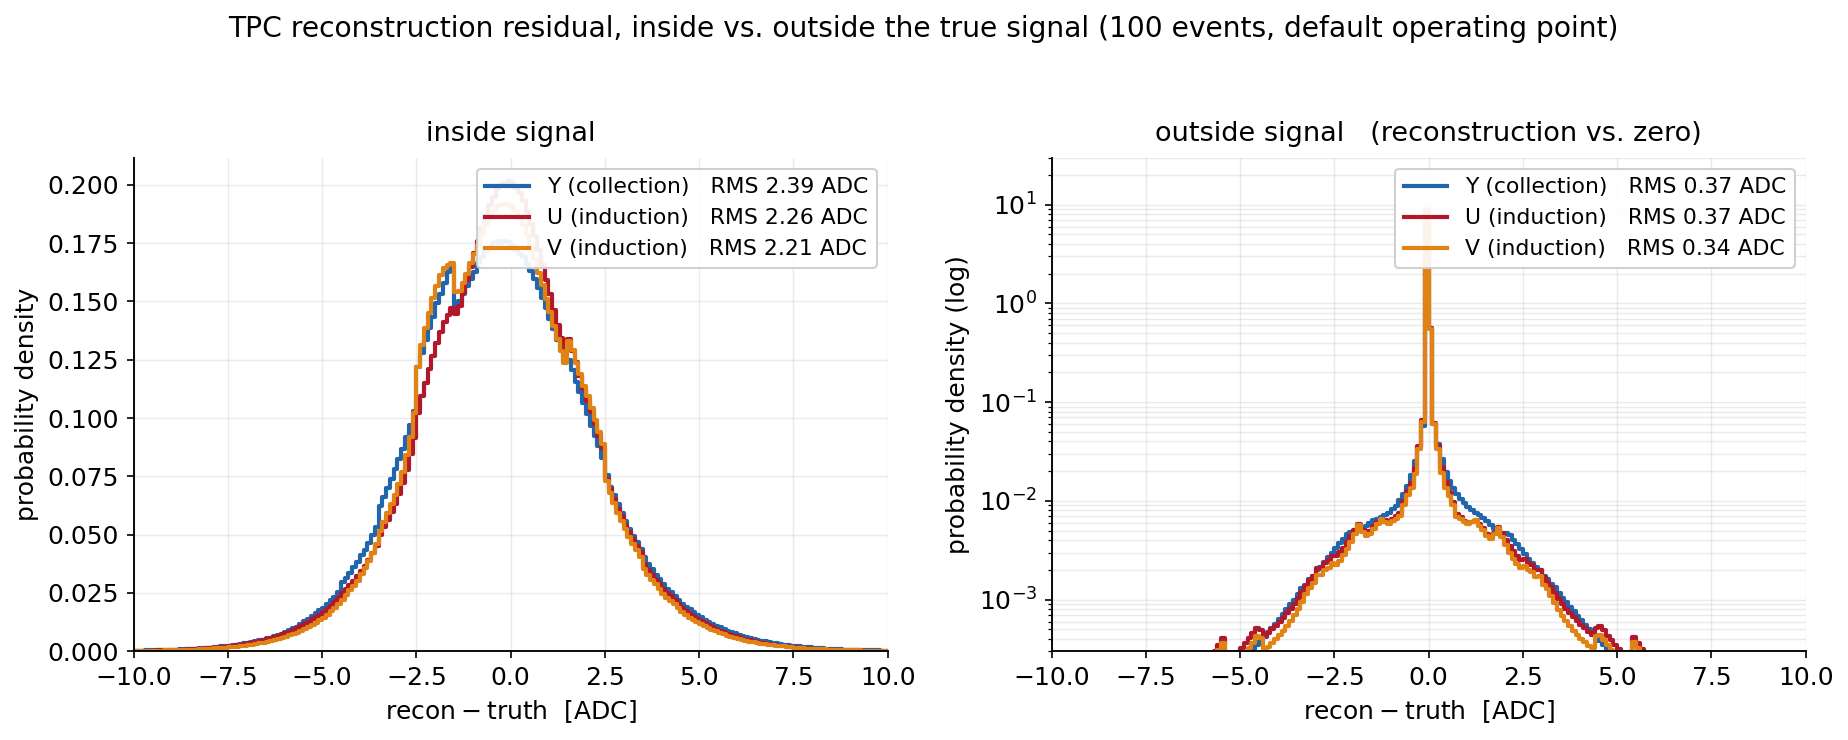
\includegraphics[width=\linewidth]{figures/tpc_resid_within_outside.png}
    \caption{\textbf{Reconstruction residual (reconstruction minus true charge)} over 100
    events, per wire plane. Left, inside the true signal: a broad distribution about 2.2--2.4
    ADC counts wide, the charge-reconstruction error on the tracks. Right, outside the true
    signal, where the true charge is zero, so the residual is the reconstruction compared to
    zero. On a logarithmic vertical scale it is a sharp peak at zero (most off-track pixels
    reconstruct to exactly zero) with rapidly falling tails: away from tracks the reconstruction
    is essentially empty.}
\end{figure}

\begin{figure}[H]
    \centering
    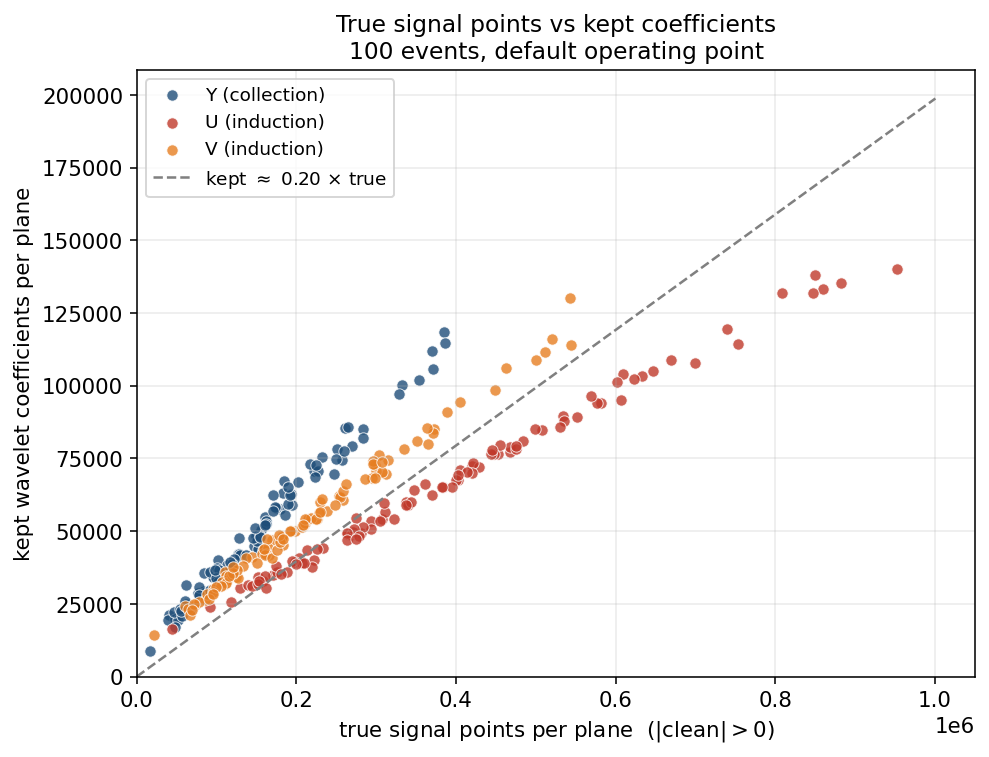
\includegraphics[width=0.72\linewidth]{figures/tpc_truepoints_vs_coeffs.png}
    \caption{\textbf{The representation scales with signal content, not raw size.} Number of
    wavelet coefficients kept versus the number of true signal points, per wire plane, over 100
    events (each marker is one plane of one event). The kept budget grows linearly with, and
    stays a few times below, the true signal size (dashed line). Relative to the full raw plane
    (about ten million pixels, mostly noise) the representation is roughly $170$--$190\times$
    more compact. Its size is set by the physics content of the event, which is what a
    token-based neural network requires.}
\end{figure}

\begin{figure}[H]
    \centering
    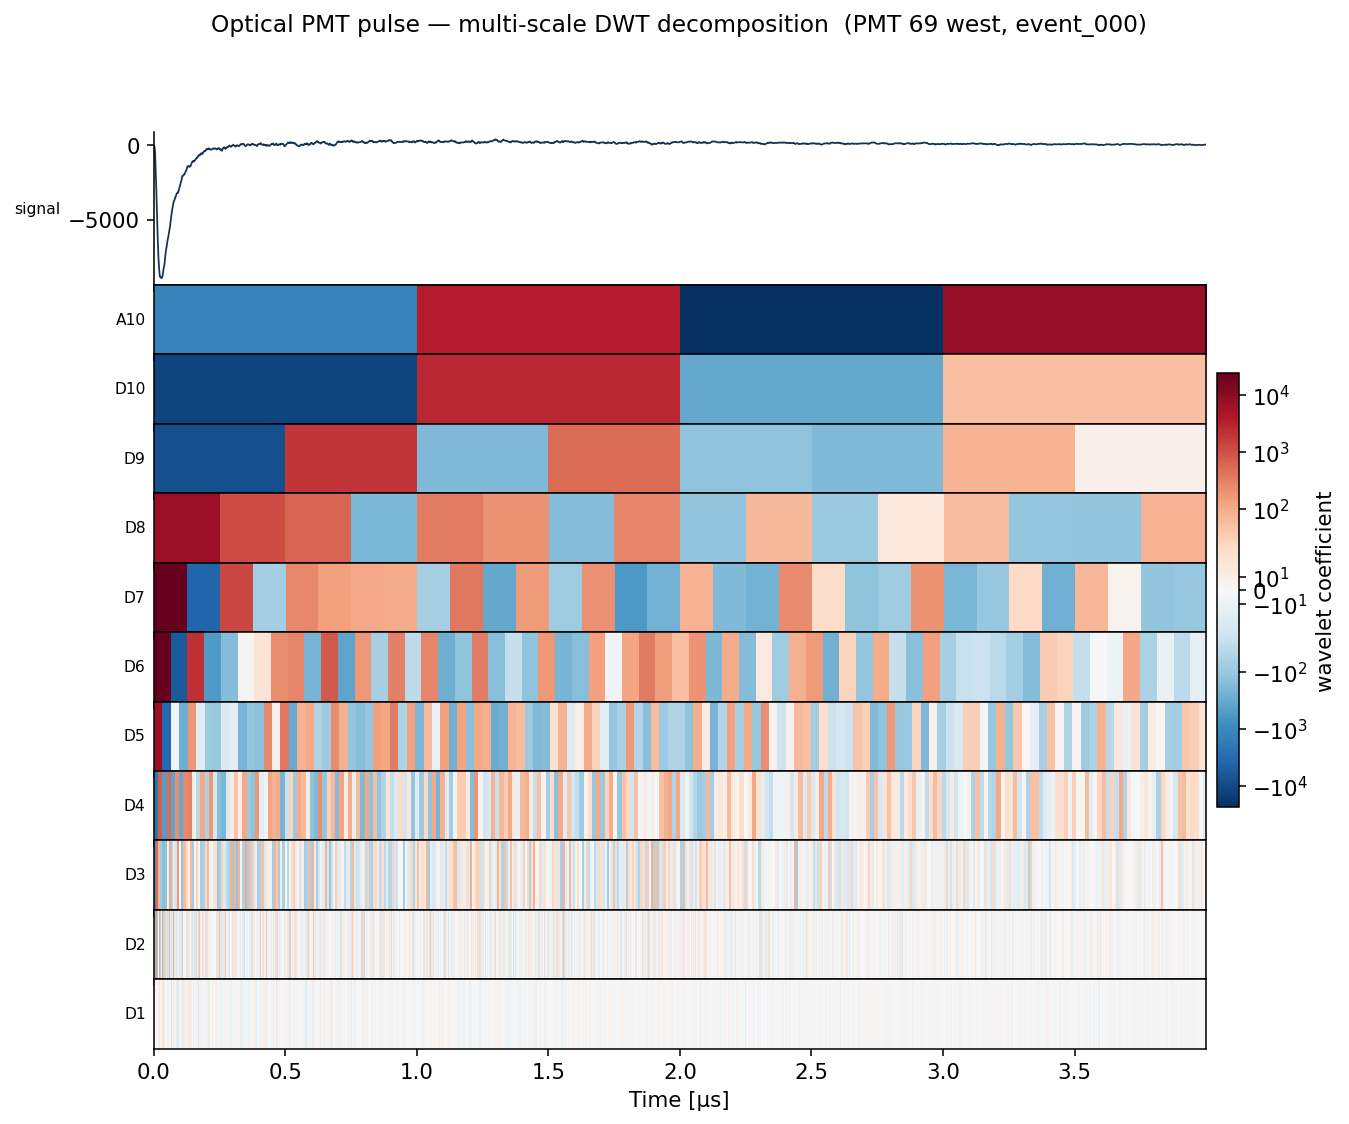
\includegraphics[width=0.78\linewidth]{figures/optical_decomposition.png}
    \caption{\textbf{Multi-scale wavelet decomposition of a single PDS light pulse.} The pulse
    energy spreads coherently across a range of time scales (rows), while the finest scale
    ($D1$, bottom) is pure noise. The compression step keeps the coefficients that stand above
    the noise and discards the noise-dominated fine scales.}
\end{figure}

\begin{figure}[H]
    \centering
    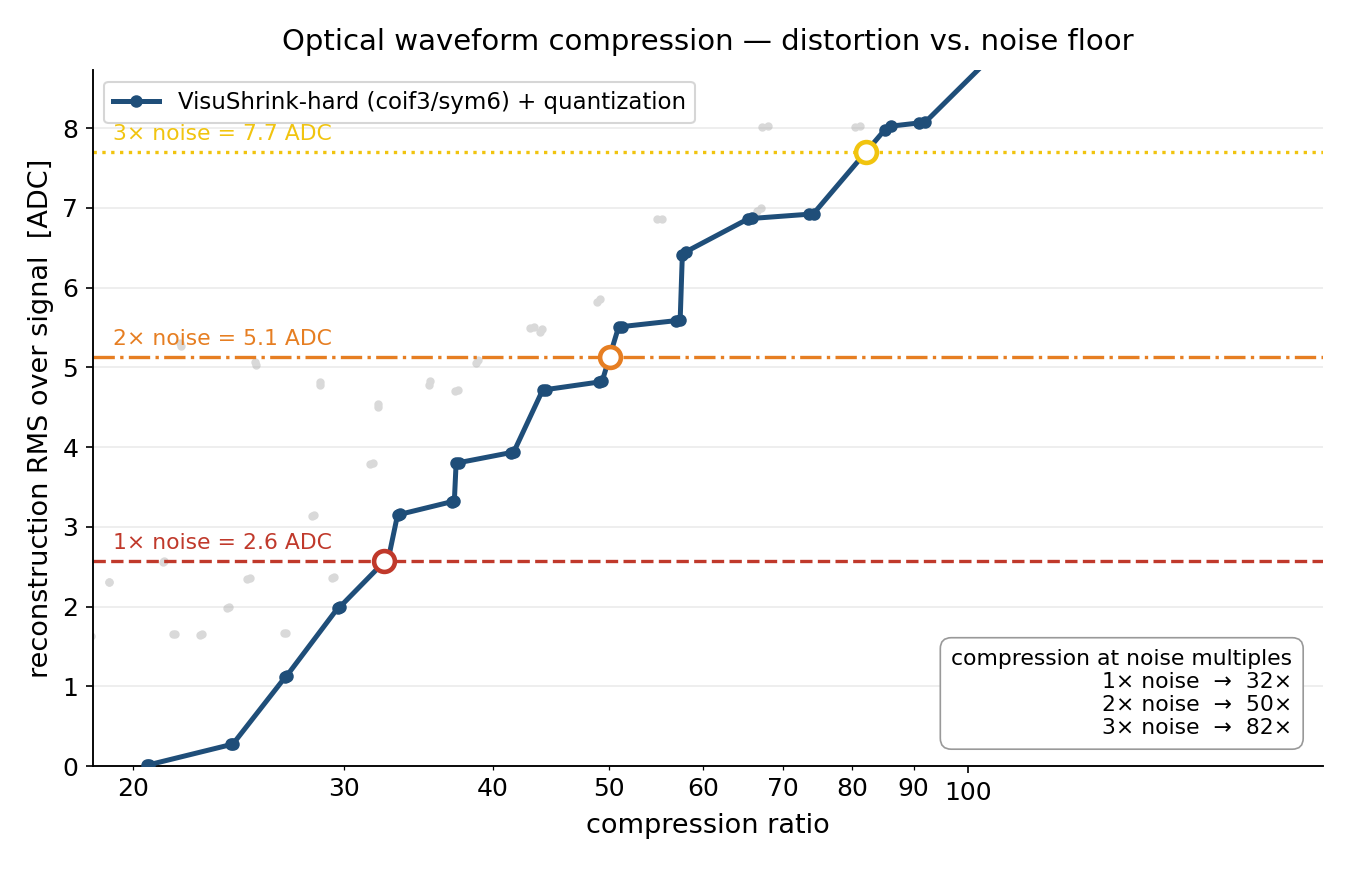
\includegraphics[width=0.82\linewidth]{figures/optical_rate_distortion.png}
    \caption{\textbf{Compression versus fidelity for the PDS waveforms.} Reconstruction error
    (RMS over the signal) against compression ratio. Horizontal lines mark one, two, and three
    times the intrinsic noise floor; the corresponding compression ratios are about
    $32\times$, $50\times$, and $82\times$. At the default operating point (one times the noise
    floor) the reconstruction error equals the noise: all information below the noise floor is
    removed essentially for free, and faithful compression is set by the noise floor rather than
    an arbitrary target.}
\end{figure}

\begin{figure}[H]
    \centering
    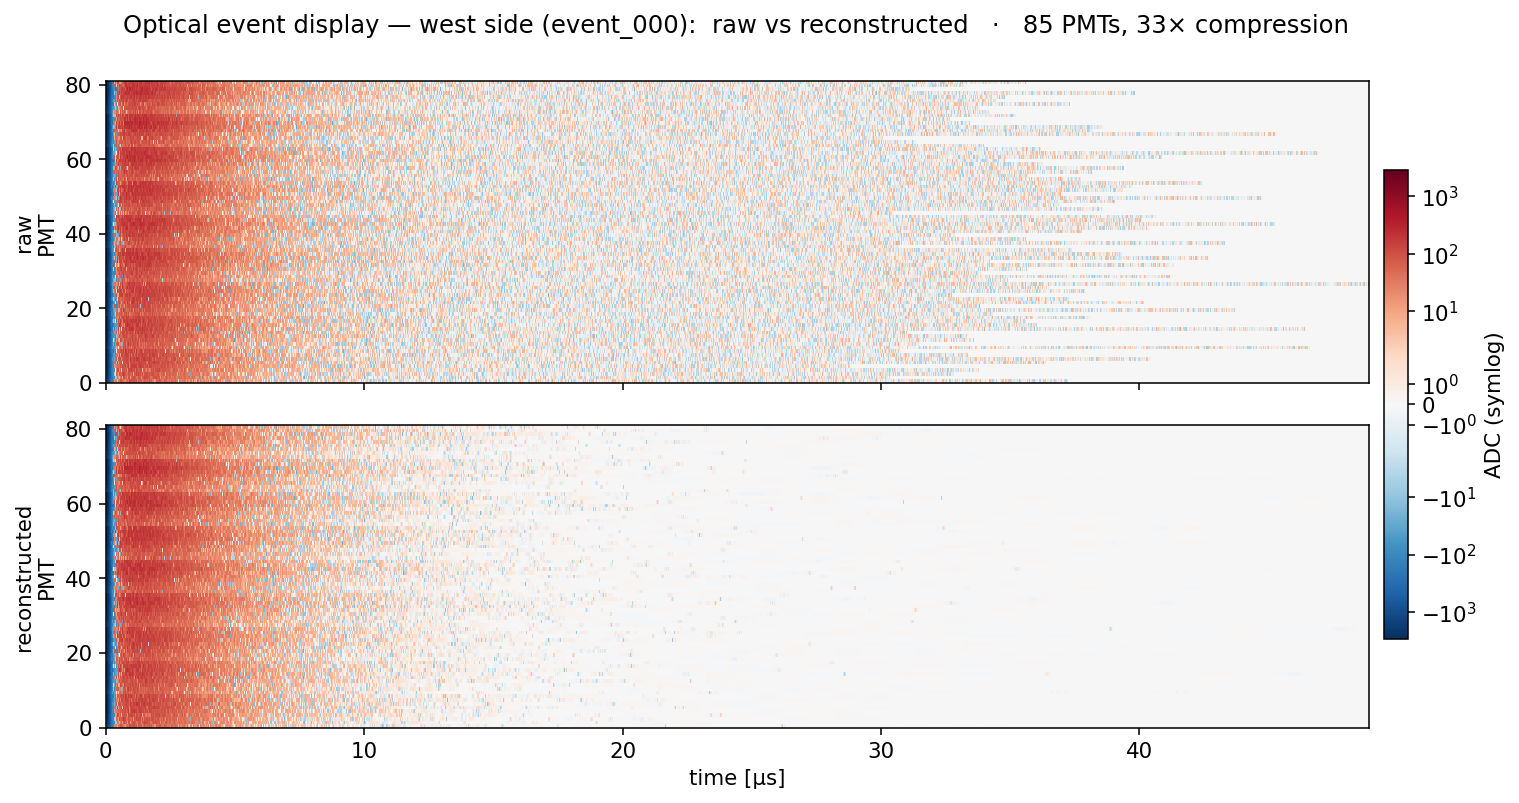
\includegraphics[width=\linewidth]{figures/optical_event_2d.png}
    \caption{\textbf{Full PDS event display} (one detector side, 85 photomultiplier tubes):
    raw waveforms (top) versus reconstruction (bottom). The prompt scintillation flash is
    preserved while the noise tail is removed, at about $33\times$ compression.}
\end{figure}

\end{document}
